% icsthesissample.tex
% UPLB Institute of Computer Science Thesis / Special Problem Template

\documentclass{icsthesis}
\usepackage{amsmath}
\usepackage{amssymb}
\usepackage{array}
\usepackage{url}
\usepackage{hyperref}
\hypersetup{
    colorlinks=true,
    linkcolor=black,
    urlcolor=black,
    citecolor=black
}

% Title and metadata settings
\renewcommand{\TITLE}{AMISYNC: PREFERENCE-AWARE COURSE-SECTION SELECTION WITH INFEASIBILITY EXPLANATION FOR UPLB AMIS USING IN-BROWSER CONSTRAINT PROGRAMMING}
\renewcommand{\AUTHOR}{DIEGO V. MEJORADA}
\renewcommand{\DEGREE}{BACHELOR OF SCIENCE}
\renewcommand{\MAJOR}{Computer Science}
\renewcommand{\MONTH}{NOVEMBER}
\renewcommand{\YEAR}{2026}

\begin{document}
	
	\begin{frontmatter}
		% Create title
		\maketitle
				
		
		% Table of Contents
		\maketableofcontents
		
		% List of Tables
		\setcounter{pagecounter}{3}
		\makelistoftables

		% List of Figures
		\setcounter{pagecounter}{4}
		\makelistoffigures

	\end{frontmatter}
	
	% BODY OF THESIS (Up to 3 levels: section -> subsection -> subsubsection)
	\begin{mainmatter}
		
		% =========================================================================
		% CHAPTER 1: INTRODUCTION
		% =========================================================================
		\section{INTRODUCTION}
		
		\subsection{Background of the Study}
		
		The efficient allocation of temporal and spatial resources is a foundational challenge in the administration of higher education. This macro-level optimization, formalized in operations research as the University Course Timetabling Problem (UCTP), defined broadly as the complex combinatorial challenge of assigning events to limited time slots and rooms without conflict \citep{chen2013, cruzrosales2022}. Traditional frameworks focus on globally distributing these resources to serve an aggregate student cohort \citep{meier2026}. While institutions utilize robust algorithms to construct these master timetables \citep{strichman2017}, the resulting environment represents a fixed, immutable matrix from the perspective of the individual student. Consequently, a parallel optimization challenge emerges at the micro-level: the student-centered course schedule optimization problem. At this level, the variables of optimization shift from institutional resource allocation to satisfying an individual student's unique academic requirements and personal constraints.
		
		To navigate this complex combinatorial solution space, students must manually balance degree requirements against subjective preferences, such as working around pre-enlisted courses, managing academic fatigue through mandated breaks, and restricting acceptable class hours. Historically, students have relied on manual trial-and-error using visual calendar interfaces. At the University of the Philippines Los Ba\~{n}os (UPLB), students utilize the Academic Management Information System (AMIS) for enrollment. To assist with the cognitive burden of manual scheduling, local third-party tools such as the AMIS Schedule Unitizer (AMISSU) browser extension were developed. These tools provide visual interfaces and facilitate basic conflict-free schedule generation through recursive combination filtering of selected courses \citep{amissu2023}.
		
		However, as digital infrastructure matures, the demand for more sophisticated decision support has grown. Advanced mathematical modeling, particularly Constraint Programming-\\Boolean Satisfiability (CP-SAT), offers exact constraint-based optimization that can prove feasibility and optimality \citep{googlecpsolver2026}. Moreover, the advent of WebAssembly (WASM) allows these previously server-bound solver engines to execute locally within the client's browser \cite{wickman2026}. This technological shift presents an opportunity to transition student-facing scheduling tools from conflict checkers into preference-aware schedule recommenders capable of immediate, localized computation.
		
		\subsection{Statement of the Problem}
		
		Students attempting to construct ideal schedules often struggle to manually balance mandatory academic constraints with highly specific personal preferences. Existing standard scheduling tools, including local systems like AMISSU, generate unranked conflict-free combinations and do not model preferences. They lack the capacity to employ structured weighted-penalty optimization to explicitly prioritize and manage complex soft constraints, such as limiting continuous class hours or minimizing Friday classes.
		
		Furthermore, when a combination of constraints, such as locked pre-enlisted courses and strict visual time blocks, makes a schedule mathematically impossible, current systems fail to provide explainable feedback. Students are left guessing why their desired schedule is infeasible. Without the computational extraction of a Minimal Unsatisfiable Subset (MUS), users are forced into an inefficient, blind trial-and-error process to resolve bottlenecks. Finally, while advanced exact solvers (like CP-SAT) exist to handle such complexities, deploying them traditionally requires centralized server infrastructure. In a high-traffic environment like the UPLB AMIS registration period, a server-side solver would add computational load to an already strained system \citep{hermocilla2022}.
		
		Therefore, this study addresses the following research gap: There is a lack of client-side decision support tools that integrate weighted-penalty preference optimization, preserve fixed pre-enlisted courses, and extract explainable infeasibility conflict sets to facilitate a human-in-the-loop schedule adjustment workflow for UPLB students.
		
		\subsection{Significance of the Study}
		
		The development and evaluation of this system yield significant benefits for several key stakeholders:
		
		\begin{itemize}
			\item \textbf{UPLB Students:} The primary beneficiaries of this study are the students, who will experience significantly reduced cognitive load during the registration period. By autonomously balancing their subjective preferences and explicitly diagnosing conflicting constraints when schedules fail, the tool empowers students to make informed, efficient academic planning decisions.
			
			\item \textbf{University Administrators and IT Infrastructure:} By compiling the heavy CP-SAT optimization engine to WebAssembly, all combinatorial computations execute locally on the student's device. This avoids the need for a server-side solver, preventing the introduction of additional computational bottlenecks to the university's centralized backend during high-traffic enlistment windows.
			
			\item \textbf{Computer Science and Operations Research Communities:} This study provides a practical, empirical application of executing exact constraint solvers (CP-SAT) via WASM for micro-level academic scheduling. It contributes to the literature on explainable scheduling by demonstrating how a Minimal Unsatisfiable Subset (MUS) can be used in a real-world, human-in-the-loop workflow without the overhead of heavy natural language processing models.
		\end{itemize}
		
		\subsection{Objectives of the Study}
		
		To develop and evaluate a preference-aware, weighted-penalty optimization decision support browser extension that generates distinct, feasible schedule alternatives and provides explainable infeasibility alerts for UPLB students.
		
		\vspace{2ex}
		\textbf{Specific Objectives:}
		\begin{enumerate}
			\item To formulate individualized class scheduling as a constraint optimization problem, translating visual time-grids, pre-enlisted status, and section preferences into hard and soft constraints to minimize a weighted-penalty objective function.
			\item To generate up to three structurally distinct, feasible schedule recommendations by applying iterative exclusion constraints.
			\item To design an Infeasibility Alert system that extracts a Minimal Unsatisfiable Subset (MUS) to pinpoint conflicting rules and guide a user-directed course substitution workflow.
			\item To evaluate algorithmic performance using reproducible static data snapshots, targeting a 100\% schedule validity rate, exact-match MUS conflict diagnosis, and an execution time of under 5 seconds to ensure acceptable human-computer interaction (HCI) responsiveness.
			\item To assess the system's effectiveness and its impact on student decision-making through a structured user evaluation, quantitatively measuring reductions in cognitive load and task completion time compared to manual scheduling.
		\end{enumerate}
		
		\subsection{Scope and Delimitation}
		
		This study encompasses the development of a browser-extension prototype designed to integrate with a student's authenticated session in the UPLB Academic Management Information System (AMIS). The system's capabilities are strictly focused on client-side schedule optimization and decision support.
		
		\subsubsection{Scope}
		The proposed system includes a user interface for preference capture, enabling interactive time-blocking, priority dropdowns for nuanced weighted preferences (such as fatigue management and day batching), and a star-to-prioritize and hide-to-exclude section selection interface. It uniquely treats pre-enlisted courses as locked, fixed variables, forcing the solver to build the remaining schedule around them. The core optimization executes locally using a WASM-based CP-SAT engine. It will generate up to three distinct schedule alternatives, ensuring each output differs by a user-defined minimum number of course-section assignments to guarantee structural diversity. If a schedule is mathematically infeasible, the system will output an Infeasibility Alert by extracting a Minimal Unsatisfiable Subset (MUS) utilizing the QuickXplain algorithm, thereby triggering a human-in-the-loop Phase 2 where the student can loosen constraints or manually input an alternative course to trigger targeted dynamic recalculation. Evaluation will be conducted using static, timestamped JSON snapshots of AMIS API data to ensure repeatable testing unaffected by live network latency, with algorithmic execution time evaluated to ensure the solver remains responsive within acceptable Human-Computer Interaction (HCI) response-time thresholds for maintaining user attention and preventing task abandonment (e.g., operating well below the 10-second absolute limit established by foundational HCI research and the modern Google RAIL performance model, targeting under 5 seconds for complex operations) \citep{miller1968, nielsen1993, googlerail2020}. Furthermore, to validate the system's impact on decision-\\making friction, a small-scale user evaluation will be conducted utilizing a standardized cognitive load metric to empirically measure reductions in user mental effort and task completion time.
		
		\subsubsection{Delimitation}
		This project is strictly a decision support tool; it does not perform automatic enlistment or enrollment on the student's behalf. It relies on retrieved course-section data but does not feature automated degree-auditing, active prerequisite validation, or curriculum guessing for course substitutions (which must be student-directed). Because the system relies on specific browser APIs, it is delimited to the desktop version of Google Chrome and does not support mobile devices. Furthermore, the temporal optimization scope is limited to standard regular semesters (excluding Midyear terms) and excludes courses with "To Be Announced" (TBA) schedules or asynchronous online modes of delivery that lack fixed time matrices. Finally, the extension operates without unrestricted access to the AMIS backend and cannot override or manipulate actual university class capacities or institutional timetabling assignments.
		
		
		% =========================================================================
		% CHAPTER 2: REVIEW OF RELATED LITERATURE
		% =========================================================================
		\section{REVIEW OF RELATED LITERATURE}
		
		\subsection{Introduction}
		
		This chapter synthesizes existing literature on the University Course Timetabling Problem (UCTP) and traces the paradigm shift towards micro-level, student-centered schedule optimization. It reviews foundational approaches to weighted-penalty preference optimization, exact constraint solving, and recent advancements in client-side WebAssembly (WASM) execution to establish the theoretical and technological justification for the proposed browser extension.
		
		\subsubsection{University Course Timetabling and Scheduling}
		The overarching optimization challenge of academic scheduling is formalized in operations research as the University Course Timetabling Problem (UCTP). The UCTP is an NP-hard combinatorial optimization problem, making large instances computationally challenging \citep{cooper1996}. Academic timetabling literature broadly bifurcates the UCTP into two distinct sub-disciplines: Post-Enrollment Course Timetabling (PE-CTP) and \\Curriculum-Based Course Timetabling (CB-CTT) \citep{meier2026}. In PE-CTP, institutions generate master schedules based on individual student enrollment data to minimize course conflicts, while CB-CTT operates on curricula groupings, introducing complex soft constraints aimed at an aggregate cohort rather than the individual \citep{chen2013, han2025}. Although these timetabling formulations account for student-related constraints to varying degrees, their primary objective is generally the construction or optimization of institutional timetables. In contrast, this study treats the institutional timetable and available course sections as a given environment and focuses on selecting a feasible combination of sections that best satisfies an individual student's preferences.
		
		\subsubsection{Student-Centered and Personalized Course Scheduling}
		To address the limitations of macro-level planning, recent paradigms have shifted toward micro-level student scheduling. In this student-centered model, the master timetable is immutable, and the student acts as the sole agent navigating a multi-dimensional matrix of overlapping times, closed sections, and personal constraints. Without automated decision support, students using legacy registration systems are frequently unable to identify the specific variables causing a schedule conflict \citep{vasileiou2025}. This lack of localized cognitive support leads to suboptimal academic planning, delayed graduation times, and highly stressful registration bottlenecks \citep{hermocilla2022}, demonstrating a critical need for student-centered tools that can search a large combinatorial solution space during human-in-the-loop schedule adjustments \citep{vasileiou2025}.
		
		\subsubsection{Student Preference-Based Scheduling}
		A robust student-facing optimizer must translate abstract visual and temporal preferences into strict mathematical parameters. In constraint programming literature, requirements are bifurcated into hard constraints (mandatory conditions) and soft constraints (prioritized user objectives) \citep{meier2026}.
		
		Within the context of student scheduling, several key features map directly to these mathematical models:
		\begin{itemize}
			\item \textbf{Visual time blocking} functions as a hard constraint, restricting the set of selectable class meeting times for selected classes.
			\item \textbf{Pre-enlisted course locking} is formulated as a hard constraint where variables for already enrolled sections are pre-assigned as fixed, unchangeable constants, forcing the algorithm to build around them.
			\item \textbf{Consecutive hours and fatigue limits} are modeled as prioritized soft constraints, applying mathematical penalties to continuous block sequences that exceed a user-defined threshold without a break.
			\item \textbf{Minimizing active days and gaps} maps to soft constraints that penalize the total number of active days on campus and idle timeslots between classes.
			\item \textbf{Minimizing Friday classes} operates as a practical, student-defined soft constraint introduced in this study's preference model by applying weighted penalties specifically to Friday time assignments.
		\end{itemize}
		
		\subsubsection{Multi-Objective Optimization in Course Scheduling}
		Because individual student preferences are frequently contradictory such as the inherent conflict between compressing a schedule into fewer days versus spreading classes evenly to minimize daily fatigue, schedulers must employ optimization strategies. Some traditional models use lexicographic optimization, a hierarchical priority method that preserves optimal values of higher-ranked objectives before evaluating lower ones \citep{rossi2006}. This system models student preferences as soft constraints integrated into a structured weighted-penalty objective function. Here, user-defined numerical weights penalize undesirable schedule attributes based on their explicit priority \citep{meier2026}.
		
		By applying iterative exclusion principles alongside these distinct preference weight configurations, systems can generate up to three distinct, feasible schedule alternatives. The iterative exclusion mechanism generates distinct schedule recommendations by adding constraints that prohibit the exact recurrence of previously generated section combinations (i.e., at least one selected course-section assignment must differ). Furthermore, meaningful diversity is encouraged by alternating or systematically re-weighting soft preference profiles across runs, rather than relying on iterative exclusion alone. This structural diversity empowers students to visually compare and weigh the trade-offs of differing layouts.
		
		\subsubsection{Algorithms and Approaches for Course Schedule Optimization}
		The choice of algorithmic approach profoundly impacts the interactive capabilities of scheduling software. Metaheuristic approaches, such as Genetic Algorithms (GA) and Particle Swarm Optimization (PSO), are commonly used to search large scheduling solution spaces. However, as heuristic search methods, they do not generally provide formal proofs of infeasibility or optimality \citep{cruzrosales2022}. Furthermore, while basic student-\\facing tools rely on unweighted recursive backtracking and permutation filtering to generate unranked schedule combinations, such approaches lack scalability and mathematical rigor when handling complex multi-objective soft constraints or providing explicit infeasibility explanations. For this study, an exact constraint-based approach is considered because it can provide feasibility and optimality guarantees under appropriate solver conditions and can support the identification of a Minimal Unsatisfiable Subset (MUS) when the model is proven infeasible.
		
		Constraint Programming--Boolean Satisfiability (CP-SAT) provides an exact constraint-\\based optimization approach and solver engine that determines feasibility or infeasibility, and can prove global optimality for a modeled combinatorial problem under sufficient computational time and resource bounds. When a scheduling model is proven infeasible, identifying the exact source of failure is critical for user-directed resolution. To achieve this, the QuickXplain algorithm \citep{junker2004} can be utilized alongside the solver to hierarchically isolate a Minimal Unsatisfiable Subset (MUS) within the constraint network. By systematically testing subsets of constraints, QuickXplain extracts an irreducible combination of conflicting section assignments, pre-enlisted courses, and user-defined time restrictions, providing highly targeted and explainable feedback for human-in-the-loop adjustments.
		
		\subsubsection{Existing University Course Scheduling Systems}
		Several large-scale institutions rely on heavy, server-side infrastructure for their academic timetabling. Centralized systems frequently deploy parallelized Boolean Satisfiability (SAT) and Constraint Satisfaction Problem (CSP) engines to process institutional and faculty constraints via web portals. Meanwhile, student-facing registration tools and third-party web platforms (such as Coursicle) provide visual schedule drafting and basic conflict detection within registration workflows \citep{coursicle}. However, the extent to which these platforms support automated, multi-objective preference optimization varies, with many existing interfaces functioning primarily as manual visual aids and basic conflict-alert wrappers.
		
		\subsubsection{Related Course Scheduling Optimization Studies}
		Recent empirical studies have attempted to bridge the gap between logical constraint solving and explainability. \citet{vasileiou2025} developed TRACE-CS, a hybrid system that combines symbolic reasoning and large language models to generate explainable course scheduling decisions. Its symbolic reasoning component produces logically grounded explanations, while its language model component translates these explanations into understandable responses. Although TRACE-CS demonstrates the potential of explainable course scheduling, the present study focuses on personalized weekly course-section selection, weighted student preferences, fixed pre-enlisted sections, and local execution within a browser extension integrated with UPLB AMIS. Furthermore, while CP-SAT engines are traditionally deployed on centralized server infrastructure to leverage heavy compute resources, they are not inherently server-bound. The recent development of WebAssembly (WASM) ports for solvers like Google OR-Tools (\texttt{or-tools-wasm}) demonstrates that heavy constraint programming can operate through local execution within the browser, providing robust computation without requiring remote execution of the optimization process \citep{wickman2026}.
		
		\subsubsection{Local Studies and Academic Scheduling Systems}
		In the Philippine context, higher education institutions frequently struggle with high-\\traffic registration periods and manual scheduling limitations. A study conducted at Central Luzon State University (CLSU) evaluated a centralized scheduling system relying on a greedy algorithm \citep{botangen2014}. While an improvement over manual plotting, the greedy algorithm executes a one-dimensional forward pattern without backtracking capabilities; if a final required course does not fit, the algorithm terminates without a complete solution, requiring manual intervention \citep{botangen2014}.
		
		At the University of the Philippines Los Ba\~{n}os (UPLB), historical context shows that registration periods frequently experience severe uptime issues due to centralized network overload, a challenge spanning both legacy systems like SAIS and the current AMIS architecture \citep{hermocilla2022}. To assist students with the current system, the AMIS Schedule Unitizer (AMISSU) was developed as a UPLB-specific Chrome extension \citep{amissu2023}.
		
		A code-level architectural analysis of AMISSU, conducted by extracting and inspecting its source code using the Chrome Extension Source Viewer tool\footnote{\url{[https://chromewebstore.google.com/detail/chrome-extension-source-v/jifpbeccnghkjeaalbbjmodiffmgedin](https://chromewebstore.google.com/detail/chrome-extension-source-v/jifpbeccnghkjeaalbbjmodiffmgedin)}}, reveals that it is implemented as a Manifest V3 browser extension utilizing Chrome's side panel and scripting APIs to inject scripts directly into authenticated UPLB AMIS sessions \citep{amissu2023}. For schedule generation, rather than employing an exact constraint solver, AMISSU utilizes a standard JavaScript recursive backtracking algorithm to evaluate permutations of selected classes, capping its maximum output at 100 generated schedules. Conflict detection is handled locally via pairwise time-overlap checks comparing course days and parsed schedule intervals.
		
		\textbf{Identified Gap:} While AMISSU automates basic conflict-free schedule generation, its codebase confirms that it lacks support for advanced individualized preference weighting (such as fatigue management and window restrictions), pre-enlisted section locking, alternative schedule diversification via iterative exclusion, and infeasibility conflict diagnosis \citep{amissu2023}. Table~\ref{table:amissu_vs_proposed} presents a structured comparison contrasting these features against the proposed WebAssembly-based CP-SAT optimization framework.
		
		\begin{table}[htbp]
		\centering
		\caption{Comparison of AMISSU and the Proposed System}
		\label{table:amissu_vs_proposed}
		\singlespacing
		\vspace{2ex}
		\begin{tabular}{|p{1.5in}|p{2.0in}|p{2.1in}|}
		\hline
		\textbf{Feature} & \textbf{AMIS Schedule Unitizer (AMISSU)} & \textbf{Proposed System} \\
		\hline
		\hline
		Conflict-free schedule generation & Supported (Recursive backtracking combination check, capped at 100 schedules) & Supported (Exact optimization via CP-SAT) \\
		\hline
		User-defined time block preferences & Not supported & Supported (Visual grid blocks modeled as hard constraints) \\
		\hline
		Weighted multi-objective soft constraints & Not supported & Supported (UI priority dropdowns map to mathematical weights for fatigue, gaps, window limits, day batching, and starred section preferences) \\
		\hline
		Strict section locking and exclusion & Not supported as optimization constraints & Supported (Pre-enlisted sections locked as fixed variables; Hidden sections constrained to zero) \\
		\hline
		Generation of multiple distinct alternatives & Permutation-based combinations (up to 100 unweighted results) & Supported via iterative exclusion and soft-preference profile alternation \\
		\hline
		Infeasibility conflict diagnosis & Not supported (codebase lacks conflict diagnosis and explanation modules) & Supported (Minimal Unsatisfiable Subset (MUS) extraction via QuickXplain) \\
		\hline
		Client-side WASM-based CP-SAT optimization & Not supported (Standard JavaScript array operations and recursion) & Supported (Native local execution via WebAssembly / \texttt{or-tools-wasm}) \\
		\hline
		\end{tabular}
		\end{table}
		
		The reviewed literature demonstrates substantial research on institutional timetabling and basic automated schedule generation. However, within the literature and systems examined in this study, limited attention has been given to integrating personalized weighted preference optimization, fixed pre-enlisted course preservation, student-directed alternative course input, and explainable infeasibility conflict sets within a client-side browser extension. Furthermore, while WebAssembly implementations demonstrate the technical feasibility of local solver execution, their application to preference-aware student scheduling in the UPLB AMIS environment remains insufficiently explored.
		
		\subsection{Theoretical Framework}
		
		This study is anchored on \textbf{Constraint Satisfaction Theory} and \textbf{Weighted-Penalty Optimization}. Constraint Satisfaction Theory models problems as a set of variables, domains, and constraints (both hard and soft). It dictates that a feasible solution space only exists when all hard constraints (e.g., non-overlapping schedules, pre-assigned fixed variables) are strictly satisfied without contradiction. As a structural design principle, section capacity filtering is handled via data preprocessing prior to optimization, rather than formulated as a mathematical model constraint. When constraints contradict, the theory enables the extraction of a Minimal Unsatisfiable Subset (MUS) to logically explain the combination of factors causing the infeasibility. Specifically, when infeasibility occurs, the system utilizes the QuickXplain algorithm to identify an irreducible set of mutually conflicting constraints (e.g., overlapping section times, locked pre-enlisted courses, or user time blocks) that cannot be simultaneously satisfied, providing a precise explanation rather than a generic error.
		
		To balance the highly subjective soft constraints of the student, \textbf{Weighted-Penalty Optimization} (or Multi-Objective Preference Optimization) is applied. This theory posits that multiple conflicting objectives can be managed through a structured weighted-penalty objective function. The solver evaluates potential schedules by assigning mathematical penalties to undesirable attributes (e.g., Friday classes, excessive gaps) scaled strictly by user-defined priority weights. The solver seeks to minimize this composite penalty score; thus, soft constraints are explicitly represented as user preferences and minimized within the weighted-penalty objective function, allowing the generation of schedules that mathematically best reflect the student's prioritized preferences.
		
		\subsection{Conceptual Framework}
		
		The system is modeled using an Input-Process-Output (IPO) architecture designed specifically for client-side execution, reducing dependence on remote solver infrastructure.
		
		\begin{itemize}
			\item \textbf{Input:} The system retrieves raw section data and capacities (the available enrollment slots at the time data is retrieved from AMIS) over the network via an external API from the university Student Information System (UPLB AMIS). It also ingests local user inputs, including visual time-grid blocks, prioritized soft constraints, intended courses, and pre-enlisted courses.
			
			\item \textbf{Process:} The computational core uses a WebAssembly (WASM)-based CP-SAT engine embedded in the browser extension to execute optimization locally. In the Base Scheduling phase, the engine translates inputs into a constraint-based mathematical model. The solver applies a structured weighted-penalty objective function to find an initial solution, followed by an iterative exclusion process to generate up to three distinct schedule alternatives for the user. If the model is mathematically infeasible, the engine leverages the QuickXplain algorithm to extract a Minimal Unsatisfiable Subset (MUS) and trigger a visual infeasibility explanation. This initiates a Human-in-\\the-Loop (HITL) adjustment phase, supporting student-initiated alternative course input to dynamically recalculate the mathematical model without acting as an automated degree auditor.
			
			\item \textbf{Output:} The system outputs up to three distinct feasible schedule recommendations presented via an interactive UI, enabling the student to evaluate structural trade-offs before executing manual registration.
		\end{itemize}
		
		\subsection{Definition of Terms}
		
		\begin{itemize}
			\item \textbf{Background/Foreground Set:} Algorithmic partitions utilized during the QuickXplain conflict extraction process. The background set contains immutable model constraints assumed to be consistent, while the foreground set contains the specific relaxable user constraints being systematically tested for conflicts.
			
			\item \textbf{Constraint Programming-Boolean Satisfiability (CP-SAT):} An exact constraint-based optimization approach and solver engine that determines feasibility or infeasibility, and can prove global optimality for a modeled combinatorial problem under sufficient computational time and resource bounds.
			
			\item \textbf{Hamming Distance:} A mathematical metric used to quantify the structural diversity between generated schedule alternatives, calculated by counting the number of differing course-section assignments between two schedules.

			\item \textbf{Hard Constraint:} A mandatory, inflexible scheduling condition that must be strictly satisfied for a schedule to be mathematically valid (e.g., temporal exclusivity, pre-assigned fixed variables).
			
			\item \textbf{Human-in-the-Loop (HITL) Adjustment:} An interactive workflow where the system halts upon detecting an infeasibility, prompting the human user to actively intervene by loosening constraints or substituting courses to resolve the bottleneck.
			
			\item \textbf{Lexicographic Optimization:} A hierarchical multi-objective optimization method that preserves the optimal values of higher-ranked objectives before evaluating lower-\\ranked ones.

			\item \textbf{Minimal Unsatisfiable Subset (MUS):} An irreducible set of mutually conflicting constraints (e.g., overlapping section times, locked pre-enlisted courses, or user time blocks) that cannot be simultaneously satisfied; utilized computationally to generate precise infeasibility explanations.

			\item \textbf{Pre-enlistment:} The administrative process wherein students secure specific course sections prior to general registration; modeled within the system as locked, fixed variables that the solver cannot alter.

			\item \textbf{Pure Satisfiability Mode:} A solver configuration that searches strictly for a mathematically feasible schedule without evaluating the weighted-penalty objective function, utilized to accelerate computational time during conflict diagnosis.

			\item \textbf{QuickXplain:} A non-intrusive divide-and-conquer algorithm used to efficiently extract a Minimal Unsatisfiable Subset (MUS) from an over-constrained problem network.
			
			\item \textbf{Schedule Diversity:} The generation of distinct schedule alternatives that offer meaningful structural differences to the user, achieved computationally through iterative exclusion constraints and the systematic alternation of soft preference profiles across runs.
			
			\item \textbf{Soft Constraint:} A flexible optimization objective that represents a user's subjective preference, modeled mathematically as a penalty applied to an objective function rather than a strict boundary.
			
			\item \textbf{University Course Timetabling Problem (UCTP):} The overarching institutional combinatorial optimization challenge of assigning university resources (rooms, faculty, time) to a set of required courses without conflict.
			
			\item \textbf{WebAssembly (WASM):} A portable binary instruction format that provides a sandboxed execution environment, allowing the CP-SAT engine to run natively and locally within the student's web browser, avoiding reliance on remote optimization servers.
			
			\item \textbf{Weighted-Penalty Optimization (or Multi-Objective Preference Optimization):} The mathematical process of evaluating potential schedules against multiple, often contradictory user objectives by integrating them into a structured objective function, where user-defined numerical weights penalize undesirable schedule attributes based on their explicit priority.
		\end{itemize}
		
		
		% =========================================================================
		% CHAPTER 3: METHODOLOGY
		% =========================================================================
		\section{METHODOLOGY}
		
		This chapter details the system architecture, mathematical formulation, algorithmic workflow, and evaluation procedures for the proposed preference-aware class schedule optimization system. Designed as a client-side browser extension for the UPLB Academic Management Information System (AMIS), the system employs Constraint Programming-\\Boolean Satisfiability (CP-SAT) to evaluate individualized scheduling models.
		
		\subsection{System Architecture and Development Environment}
		
		The system is constructed based on an Input-Process-Output (IPO) architecture designed to execute heavy combinatorial optimization locally on the client's machine, thereby circumventing the latency and server-load vulnerabilities typical of centralized academic registration systems. The system's logical flow is illustrated in Figure~\ref{fig:ipo_architecture}, depicting the continuous data flow from the AMIS API to the React frontend, through state preprocessing, into the WASM worker, and ultimately returning the optimized schedules.
		
		\begin{figure}[htbp]
		\centering
		\vspace{2ex}
		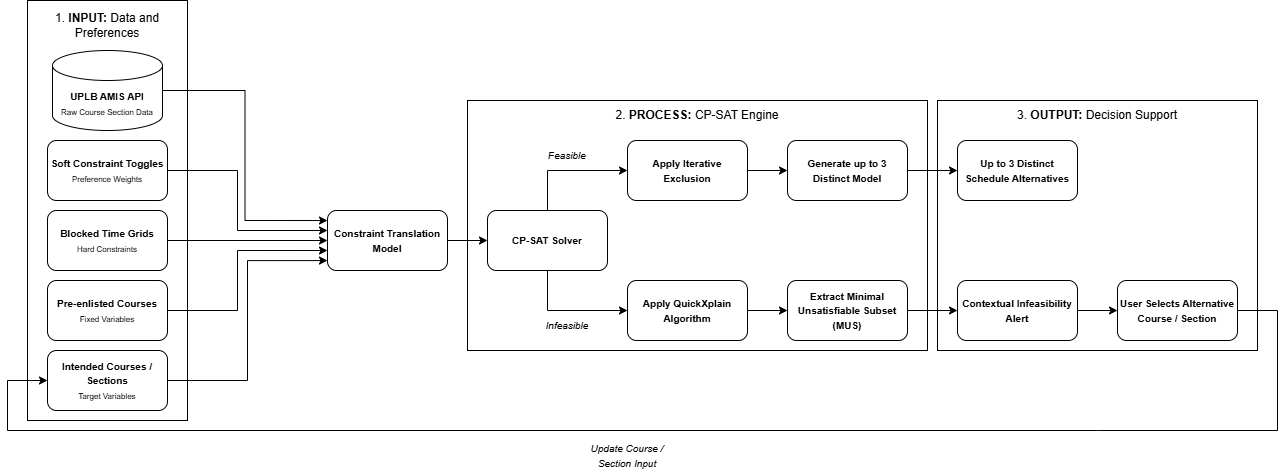
\includegraphics[width=1\textwidth]{IPO.png}
		\caption{Input-Process-Output (IPO) architecture of the client-side scheduling browser extension}
		\label{fig:ipo_architecture}
		\end{figure}
		
		The architecture consists of three primary components:
		
		\begin{enumerate}	
			\item \textbf{Input (Data Retrieval and Preference Capture):} The browser extension acts as the client interface, injecting a UI layer built as a Single Page Application (SPA) using React and Vite, compiled specifically to comply with Chrome Extension Manifest V3 strict Content Security Policies (CSP). It retrieves raw course and section data via targeted API fetches. User preferences (time blocks, slider weights) are stored in \texttt{chrome.storage.local} to maintain state across sessions without transmitting personal data to external databases.

            \begin{figure}[htbp]
    		\centering
    		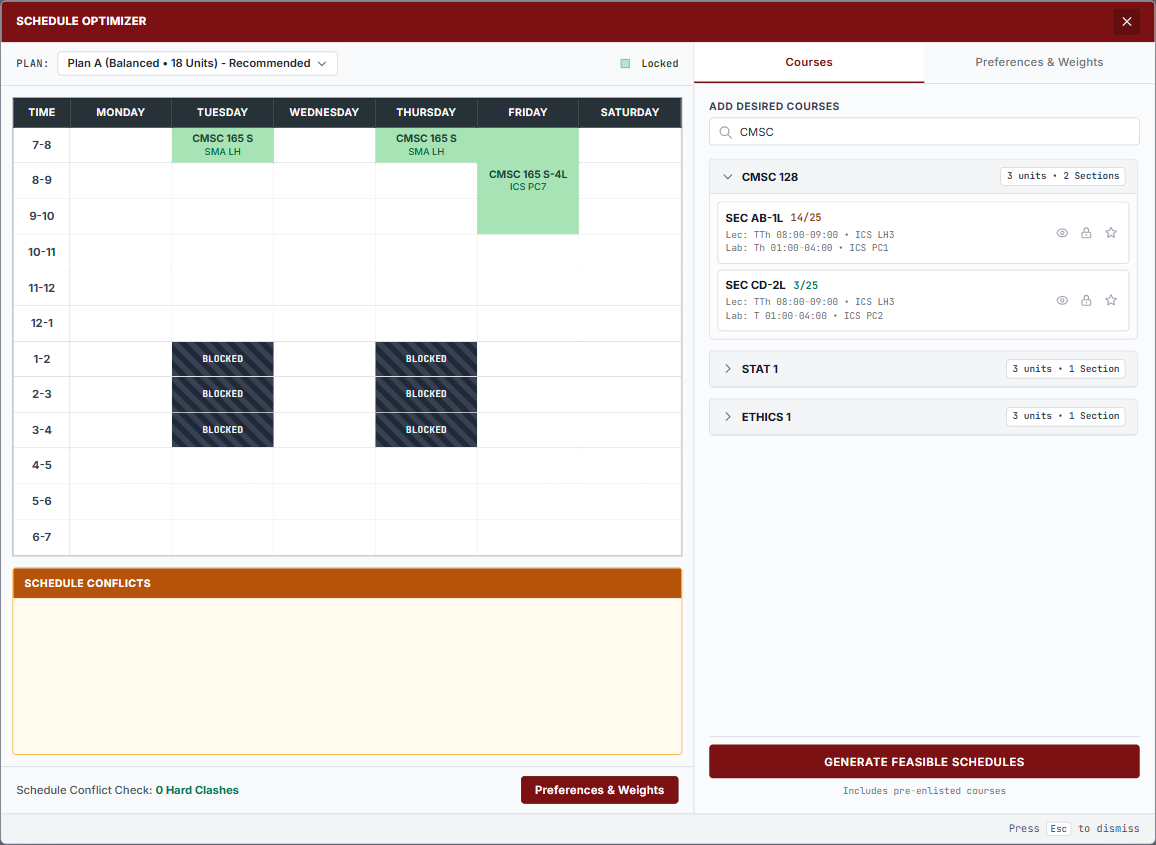
\includegraphics[width=1\textwidth]{1.1.png}
    		\caption{Interface displaying the Courses tab, enabling users to retrieve section availability, select intended courses, and manually block specific time intervals on the visual grid.}
    		\label{fig:courses_tab}
    		\end{figure}
			
			\item \textbf{Process (WASM-Based CP-SAT Engine):} To prevent main-thread blocking in the browser, the React application serializes the normalized AMIS data and passes it to a WebAssembly Web Worker running Google OR-Tools (\texttt{or-tools-wasm}). The engine mathematically translates the inputs into a weighted-penalty model. If feasible, it utilizes the QuickXplain algorithm to return a minimal conflict, represented as a Minimal Unsatisfiable Subset (MUS) \citep{junker2004}.
			
			\item \textbf{Output (Interactive Decision Support):} The Web Worker returns a JSON payload of the optimized section IDs back to the React UI, which renders up to three distinct schedule alternatives. In the event of an unsolvable model, it outputs an Infeasibility Alert, detailing the conflicting constraints and prompting a human-in-the-loop workflow.

            \begin{figure}[htbp]
                \centering
                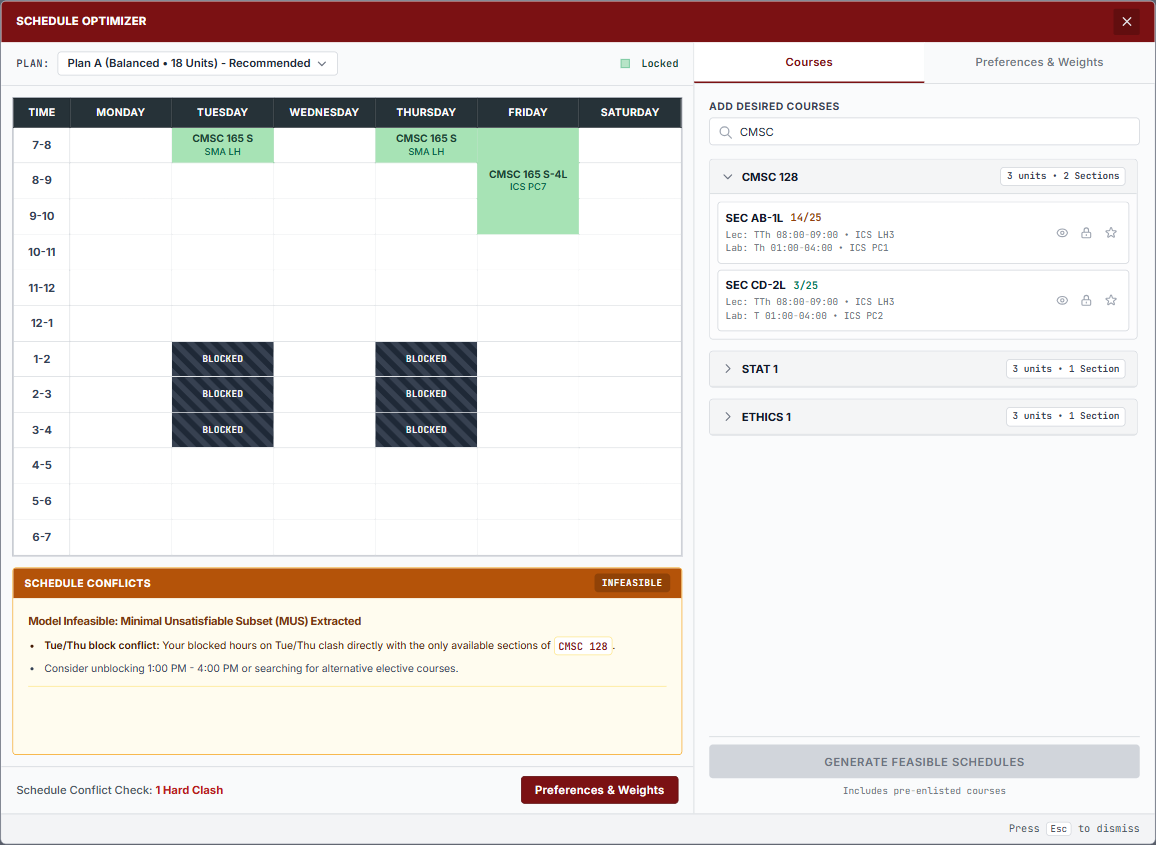
\includegraphics[width=1\textwidth]{2.0.png}
                \caption{Infeasibility Alert generated via the QuickXplain algorithm, dynamically extracting and displaying a minimal unsatisfiable subset (MUS) conflict between the user's temporal constraints and section availability.}
                \label{fig:infeasibility_alert}
            \end{figure}

			As illustrated in Figure 3, once the QuickXplain algorithm isolates the Minimal Unsatisfiable Subset (MUS), the system must translate this mathematical conflict into actionable user feedback. To generate the relaxation suggestion, the frontend implements a deterministic mapping mechanism. It parses the specific constraint variables trapped within the MUS—such as the exact array of user-defined time blocks and the specific course IDs lacking available sections outside those blocks—and passes them into predefined natural-language templates. This translates raw boolean conflicts into targeted, human-readable advice (e.g., explicitly advising the student to unblock a specific time window or drop a specific elective), guiding the user toward restoring model feasibility.
		\end{enumerate}
		
		\subsection{Mathematical Formulation of the Scheduling Problem}
		
		To enable exact computational reasoning, the micro-level student scheduling problem is formulated as a Constraint Satisfaction Problem (CSP) optimized via a weighted-penalty objective function \citep{rossi2006}.
		
		\subsubsection{Decision Variables and Pre-enlisted Courses}
		
		To accurately represent UPLB's multi-component courses, the fundamental decision variable is a Boolean, $x_{c,k,s} \in \{0, 1\}$, where $x_{c,k,s} = 1$ if section $s$ of component $k$ (e.g., Lecture, Laboratory) for course $c$ is selected, and $0$ otherwise.
		
		To strictly enforce pre-enlisted courses as immutable anchors, the system initializes pre-enlisted sections as fixed constants rather than open variables. If a student is already enrolled in a Lecture section $p$ and a corresponding Laboratory section $q$, the solver explicitly pre-assigns both components:
		\begin{equation}
		x_{c,\text{LEC},p} = 1 \quad \text{and} \quad x_{c,\text{LAB},q} = 1
		\end{equation}
		This drastically prunes the combinatorial search space. Crucially, locking a pre-enlisted lecture to $1$ mathematically forces the solver to evaluate the corresponding child components based on the co-requisite linkage constraints defined below.
		
		\subsubsection{Hard Constraints}
		
		Hard constraints define the rigid boundaries of a mathematically valid schedule. A schedule is considered infeasible if any of the following are violated:
		
		\begin{itemize}
			\item \textbf{Component Satisfaction:} For every required component $k$ of an intended course $c$, exactly one section must be selected:
			\begin{equation}
			\sum_{s} x_{c,k,s} = 1
			\end{equation}
			The system determines which components are mandatory during the preprocessing phase by analyzing the component arrays in the AMIS API payload. If a course entry contains multiple component types (e.g., Lecture and Laboratory), they are treated as mandatory co-requisites. Optional components are excluded from this strict requirement unless explicitly requested.
			
			\item \textbf{Component Co-requisite Linkage:} AMIS structures course components relationally. If the solver selects a parent lecture section $p$, and a laboratory component is required, it must strictly evaluate and select exactly one child laboratory section $l$ from the set of compatible sections sharing the corresponding \texttt{parent\_class\_id}:
			\begin{equation}
			\sum_{l \in \text{child}(p)} x_{c,\text{LAB},l} = x_{c,\text{LEC},p}
			\end{equation}
			For courses featuring multiple possible parent-child component combinations (e.g., a lecture requiring a distinct laboratory), the solver enforces cascading linkage constraints where each required child component type must independently satisfy the equation above relative to the selected parent node.
			
			\item \textbf{Temporal Exclusivity:} No two selected sections can share overlapping time intervals on any shared meeting day. Using minutes since midnight as a continuous integer scale (0 to 1440), two sections $i$ and $j$ that share at least one meeting day overlap if and only if:
			\begin{equation}
			start_i < end_j \quad \land \quad start_j < end_i
			\end{equation}
			This ensures that adjacent classes (where $end_i = start_j$) are correctly identified as non-overlapping. To strictly enforce this, for every overlapping pair of sections $i$ and $j$ (including pre-enlisted sections), the solver applies the following constraint:
			\begin{equation}
			x_i + x_j \leq 1
			\end{equation}

			\item \textbf{User-Excluded Sections (Hide):} If a user explicitly hides or excludes a section $s$ using the interface, that specific section is strictly forbidden from being selected. The solver permanently locks its decision variable:
			\begin{equation}
			x_{c,k,s} = 0
			\end{equation}
			
			\item \textbf{User Time-Blocks:} Sections intersecting with the user's manually blocked visual grid are strictly forbidden. If section $s$ overlaps with a blocked period on a given day, it is constrained as:
			\begin{equation}
			x_{c,k,s} = 0
			\end{equation}
		\end{itemize}
		
		\subsubsection{Soft Constraints and Weighted-Penalty Objective Function}

		\begin{figure}[htbp]
            \centering
            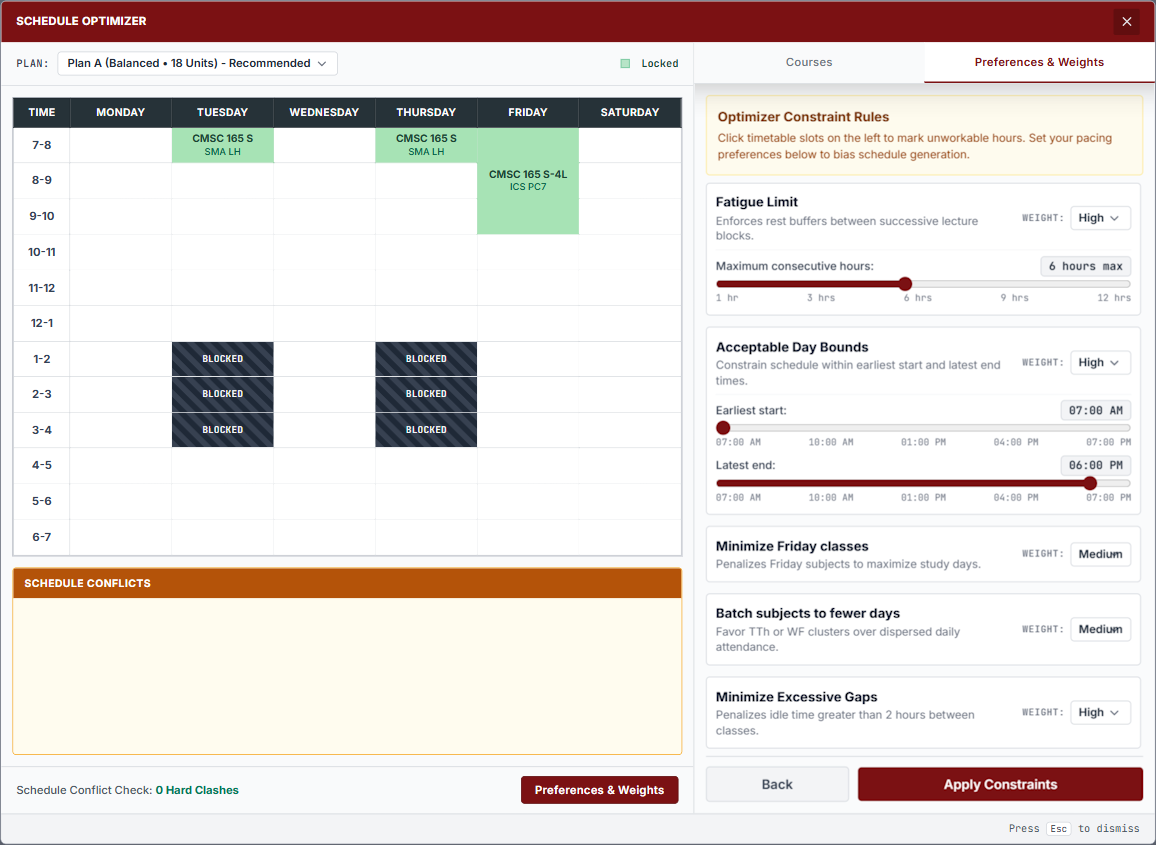
\includegraphics[width=1\textwidth]{1.2.png}
            \caption{The Preferences and Weights configuration panel, where users define the priority of soft constraints for the CP-SAT weighted-penalty objective function.}
            \label{fig:preferences_tab}
        \end{figure}

        The system utilizes a structured weighted-penalty optimization model \citep{rossi2006}. As reflected in the graphical user interface, users assign a priority level to each preference via a dropdown menu (e.g., Off, Low, Medium, High). These UI selections are mapped to a mathematical weight variable $W_n \in \{0, 2, 5, 10\}$ for each preference $n$, dictating how heavily the solver penalizes violations of that rule.\\

		\textbf{Zero-Weight Exception:} If all preference weights are set to zero ($\Sigma W = 0$), the objective function $Z$ is simply set to 0. The solver then operates in Pure Satisfiability Mode, searching solely for any mathematically feasible configuration that satisfies the hard constraints.

		When $\sum W > 0$, the raw penalties ($P_{\text{raw}}$) are mapped to a normalized scale $P'_n \in [0, 1]$ using max-normalization. The theoretical maximum penalty ($P_{\text{max}}$) used for normalization is calculated dynamically based on the student's specific input bounds.

		The raw penalty formulas are defined as follows:
		\begin{itemize}
			\item \textbf{Early Start Penalty:} Evaluates only the \textit{first} class of each day $d$ against the user's slider threshold ($T_{\text{pref\_start}}$):
			\begin{equation}
			P_{\text{early}} = \sum_{d} \max\left(0, T_{\text{pref\_start}} - \min_{c \in d}(start_c)\right)
			\end{equation}
			
			\item \textbf{Late End Penalty:} Evaluates only the \textit{last} class of each day $d$ against the user's slider threshold ($T_{\text{pref\_end}}$):
			\begin{equation}
			P_{\text{late}} = \sum_{d} \max\left(0, \max_{c \in d}(end_c) - T_{\text{pref\_end}}\right)
			\end{equation}
			
			\item \textbf{Friday Class Penalty:} Adds a discrete penalty for every individual class scheduled on a Friday:
			\begin{equation}
			P_{\text{friday}} = \sum_{c} (x_c \cdot I_{\text{Friday}}) \quad \text{where } I_{\text{Friday}} = \begin{cases} 1 & \text{if section meets on Friday} \\ 0 & \text{otherwise} \end{cases}
			\end{equation}

			\item \textbf{Active Days Penalty (Batching Subjects):} Penalizes schedules that spread classes across too many days, inherently favoring compressed schedules:
			\begin{equation}
			P_{\text{days}} = \sum_{d} y_d \quad \text{where } y_d = \begin{cases} 1 & \text{if } \sum_{c \in d} x_c > 0 \\ 0 & \text{otherwise} \end{cases}
			\end{equation}

			\item \textbf{Consecutive Hours Penalty (Fatigue Limit):} Penalizes continuous blocks of classes that exceed the user's slider threshold ($T_{\text{fatigue}}$) without a break. Let $B_{d, k}$ be the total duration of the $k$-th continuous back-to-back class block on day $d$:
			\begin{equation}
			P_{\text{fatigue}} = \sum_{d} \sum_{k} \max\left(0, B_{d, k} - T_{\text{fatigue}}\right)
			\end{equation}

			\item \textbf{Section Preference Penalty (Star):} Applies a penalty if the solver is forced to select a section that the user did not explicitly star (prioritize) in the UI:
			\begin{equation}
			P_{\text{section}} = \sum_{s} (x_s \cdot I_{\text{unstarred}}) \quad \text{where } I_{\text{unstarred}} = \begin{cases} 0 & \text{if section } s \text{ is starred} \\ 1 & \text{otherwise} \end{cases}
			\end{equation}
			
			\item \textbf{Excessive Gap Penalty:} Penalizes idle time between consecutive classes on the same day. Using day-specific auxiliary variables $y_{i,j,d}$ (evaluating to 1 if sections $i$ and $j$ are consecutive on day $d$):
			\begin{equation}
			P_{\text{gap}} = \sum_{d} \sum_{i,j} y_{i,j,d} \cdot \max(0, (start_{j} - end_i) - 120)
			\end{equation}
		\end{itemize}

		The CP-SAT engine minimizes the composite objective function, Z. Because CP-SAT requires integer coefficients for its objective function, each individual normalized weight coefficient is multiplied by a scaling factor (10,000) and rounded to the nearest integer before summation. This preserves the relative fractional importance of the weights while satisfying the solver's integer constraint:
		\begin{equation}
		\text{Minimize } Z = \sum_{n} \left[ \text{Round}\left(10000 \cdot \frac{W_n}{\sum W}\right) \cdot P'_n \right], \quad \text{for } \sum W > 0
		\end{equation}
		
		\subsection{Algorithmic Workflow and Application Features}

        \begin{figure}[htbp]
            \centering
            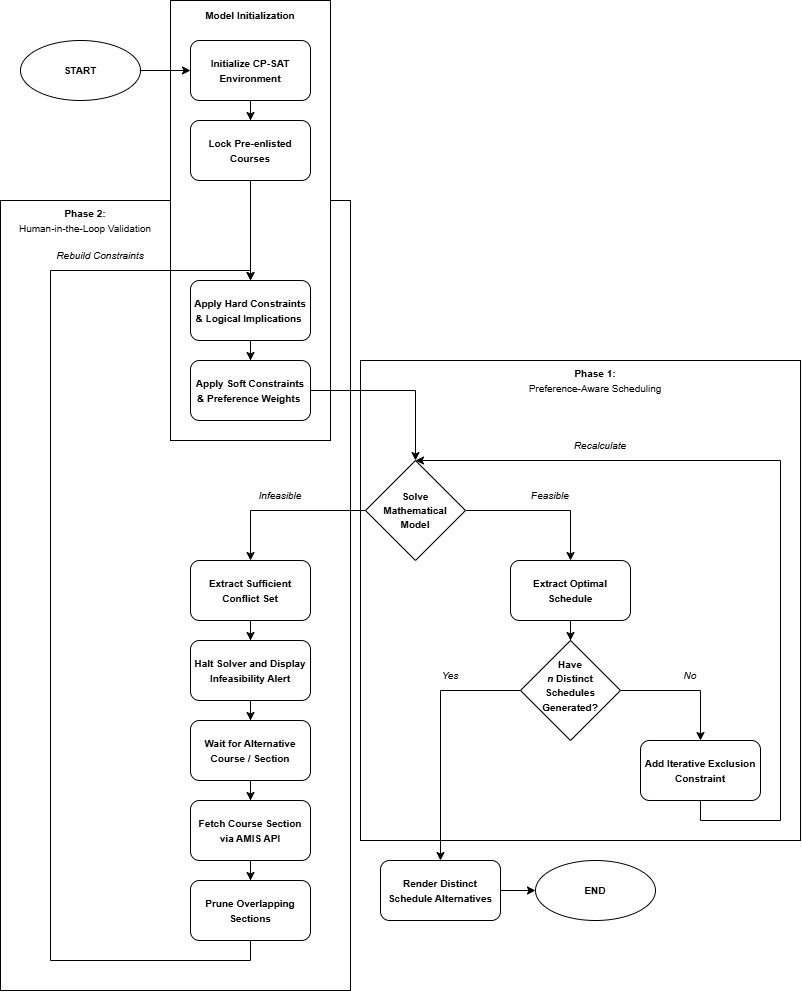
\includegraphics[width=1\textwidth]{Decision-Tree.png}
            \caption{Algorithmic workflow and decision tree of the CP-SAT scheduling engine.}
            \label{fig:decision_tree}
        \end{figure}
		
		\subsubsection{Phase 1: Preference-Aware Base Scheduling and Iterative Exclusion}
		In Phase 1, the WebAssembly CP-SAT engine attempts to find a schedule minimizing the objective function. If the solver proves mathematical optimality, it returns an \texttt{OPTIMAL} status. If the solver hits a predefined heuristic time limit (e.g., 10.0 seconds) utilizing 1 search worker, but has found at least one valid schedule, it returns a \texttt{FEASIBLE} status. Both statuses are presented to the user, though \texttt{FEASIBLE} results are distinctly labeled as such to indicate that a mathematically superior permutation might theoretically exist.
		
		When a schedule $S_i$ is generated, the system dynamically injects an iterative exclusion constraint to prevent the solver from returning highly similar permutations. To enforce structural schedule diversity, the solver requires that each subsequent alternative must differ from all previously generated schedules by at least $m$ selected sections, where $m$ is a tunable diversity parameter (e.g., $m=2$ forces the solver to replace at least two distinct sections). 

		To ensure subsequent schedules do not revert to earlier permutations, the solver maintains an accumulating set of exclusion constraints for \textit{every} previously generated schedule. Pre-enlisted sections are omitted from this calculation so they do not interfere with alternative generation. Additionally, if adding this exclusion cut makes the updated model mathematically infeasible, the system gracefully halts iteration and returns the valid schedules found so far (from Figure 5). The constraint is defined as:
		\begin{equation}
		\sum_{(c,k,s) \in S_i, s \notin \text{pre-enlisted}} x_{c,k,s} \le |S_i \setminus \text{pre-enlisted}| - m
		\end{equation}

		By utilizing the diversity parameter $m$, the mathematical model natively guarantees the structural distinctness of the generated alternatives. The system loops this exclusion process to return up to three distinct schedule recommendations, after which Phase 1 gracefully halts to preserve client-side computational resources.
		
		\textbf{Schedule Diversity:} While the iterative exclusion constraint mathematically guarantees each generated alternative differs by at least one selected decision variable, it does not guarantee the schedules are meaningfully different to the user. To enforce and evaluate schedule diversity, the system calculates the Hamming distance between the sets of selected boolean variables ($x_{c,k,s}$) of the generated schedules, strictly excluding fixed pre-enlisted sections. 
		
		By enforcing Equation 12, the system mathematically guarantees a minimum Hamming distance of $D \geq 2$ between generated schedules. Because selecting one section instead of another inherently changes two boolean variables (the previously selected section flips from 1 to 0, and the newly selected section flips from 0 to 1), this distance represents the baseline diversity of at least one complete section replacement. If a stricter, more meaningful structural diversity criterion is enforced (e.g., requiring multiple courses to differ, such that $D \geq 4$), and a generated schedule fails this threshold, the alternative is discarded. To yield a sufficiently diverse option, the solver does not dynamically resume a previous search branch; rather, the system initiates a complete re-run of the model appended with an updated exclusion cut.
		
		\subsubsection{Phase 2: QuickXplain Infeasibility Resolution}
		
		If the model is \texttt{INFEASIBLE}, Phase 2 triggers conflict diagnosis utilizing the QuickXplain algorithm \citep{junker2004}.
		
		To ensure accurate diagnosis, the system differentiates conflict origins before invoking the extraction algorithm:\\
		\begin{enumerate}
			\item \textbf{Data Inconsistency:} The system first evaluates the immutable Background Set. Because temporal exclusivity and co-requisite linkage alone are trivially satisfiable (i.e., yielding a valid model if all decision variables $x=0$), the Background Set is precisely defined to include these structural rules alongside mandatory component satisfaction requirements and locked pre-enlisted courses. If this foundational set is inherently inconsistent, the system flags a foundational data error.
			\item \textbf{Exhausted Capacity:} If an intended course has zero available sections across all its permutations, this is caught during preprocessing and flagged as an unavailable course, rather than a preference conflict.
			\item \textbf{Preference Conflict:} If the first two checks pass, QuickXplain is utilized to isolate the genuine conflicting subset within the relaxable Foreground Set. This set is precisely defined as the user's adjustable inputs: the specific intended courses targeted for enrollment and visually drawn time-blocks.
		\end{enumerate}
		
		Implementation of this phase relies on the \texttt{or-tools-wasm} compilation supporting rapid model rebuilding and repeated feasibility checks. To account for potential system failures within sandboxed browser memory limits, a fallback mechanism is established: if the engine exceeds memory bounds or times out during recursive consistency checks, the extraction aborts and returns a standard generic infeasibility error, prompting the user to manually remove constraints. Otherwise, the algorithm successfully performs recursive consistency checks on the foreground constraints. It systematically isolates a minimal conflicting subset of the user's constraints that is unsatisfiable as a whole relative to the consistent background set. While this subset is irreducible (removing any single constraint within it restores satisfiability), QuickXplain returns \textit{a} valid MUS, which is not guaranteed to be the absolute Smallest Minimal Unsatisfiable Subset (SMUS). To ensure deterministic extraction and prioritize the student's most critical preferences, the system enforces a strict ordering policy prior to execution: foreground constraints are sorted sequentially based on their user-defined priority weights (from highest to lowest priority). This guarantees that the algorithm systematically evaluates and attempts to preserve the user's most valued constraints first before identifying the conflicting subset.
		
		\subsection{Data Handling and Preprocessing}
		
		\begin{itemize}
			\item \textbf{Time Matrix Conversion:} String timestamps (e.g., ``08:00 AM'') are parsed into continuous integers representing minutes since midnight ($0$ to $1440$). Multiple meeting days are handled by applying these minute intervals across day-specific evaluation matrices.
			
			\item \textbf{Capacity Pruning:} The system evaluates \texttt{active\_class\_size} against \texttt{max\_class\_size} and drops any section with zero available slots before generating Boolean variables. Pre-enlisted sections are strictly exempted from this pruning rule, as a section the student already holds may legitimately reflect zero remaining slots. Because this occurs client-side, the system explicitly acknowledges that this availability is a transient point-in-time snapshot; live AMIS availability may shift rapidly between optimization and the student's actual enlistment action.
		\end{itemize}
		
		\subsection{Evaluation Metrics and Experimental Setup}
		
		The system will be evaluated against an AMISSU-like exhaustive backtracking baseline. To ensure rigorous comparability, both algorithms will process the exact same static JSON data snapshots and execute on identical hardware architectures.
		
		This baseline implements a standard backtracking search strategy utilizing basic forward checking as a pruning mechanism, immediately abandoning branches that violate temporal exclusivity or capacity limits. The baseline algorithm will run continuously until it exhausts its search tree or hits a stopping condition equal to the CP-SAT engine's predefined heuristic time limit. While the DFS algorithm generates schedules purely through satisfiability without guiding its search via heuristics, all resulting valid schedules will be retroactively evaluated using the same composite objective function ($Z$) applied to the CP-SAT engine to ensure parity in schedule quality comparison.
		
		\textbf{Reproducibility and Experimental Setup:}
		To ensure defensible benchmarking, the experimental environment is strictly defined:
		\begin{enumerate}
			\item \textbf{Hardware:} 12th Gen Intel(R) Core(TM) i5-1235U (1.30 GHz) processor with 8.00 GB RAM.
			\item \textbf{Software:} 64-bit Windows operating system, executing within Google Chrome version 157.0.8103.51 (Manifest V3 compliant). To simulate performance on lower-tier hardware, testing includes evaluation under a 4x CPU-throttled profile configured via Chrome DevTools.
			\item \textbf{Toolchain:} Google OR-Tools WebAssembly port (v9.x).
			\item \textbf{Datasets:} Five distinct, static JSON snapshots mapped across three scalability tiers (Low, Medium, and High Complexity) to represent varying degrees of constraint complexity. These datasets were derived from historical AMIS data obtained through voluntary student submissions of their local AMIS scheduling data. To ensure privacy, all data was strictly anonymized prior to testing, stripping identifying student information while preserving structural course relationships and capacities. The datasets explicitly document the exact number of sections, required components per course, the distribution ratio of available versus fully-booked sections, and the number of fixed pre-enlisted anchor courses included in each test case.
			\item \textbf{Trial Execution:} 30 independent trials per scenario using identical datasets, run in a randomized execution order to mitigate thermal throttling bias. Performance metrics will be evaluated using the Wilcoxon signed-rank test to determine statistical significance, with results reported as medians alongside the Interquartile Range (IQR) to account for execution time variance and browser-level outliers.
			\item \textbf{Profiling Scope:} Execution time explicitly tracks WASM initialization as an independent sub-metric to isolate the engine cold-start delay from the actual mathematical solving time.
		\end{enumerate}
		
		\vspace{2ex}
		\textbf{Algorithmic Evaluation Metrics:}
		\begin{enumerate}
			\item \textbf{Schedule Validity Rate (SVR):} An independent algorithmic validator script will evaluate every generated schedule post-execution to mathematically verify zero temporal overlaps, intact parent-child linkages, and valid capacity. Target: 100\%.
			\item \textbf{Execution Time Profiling:} Total processing time will be profiled into Data Retrieval, Model Construction, Solver Execution, and Result Rendering, maintaining a median solver execution under 5.0 seconds as a project performance target.
			\item \textbf{Schedule Quality and Baseline Comparison:} The objective score ($Z$) of each generated schedule, the terminal status returned by CP-SAT (\texttt{OPTIMAL} vs. \texttt{FEASIBLE}), and the total number of valid schedules generated will be directly compared between CP-SAT and the DFS baseline.
			\item \textbf{Conflict Diagnosis Accuracy:} Because multiple valid MUS solutions can exist for a given constraint network, QuickXplain accuracy is evaluated by constructing test scenarios specifically designed to yield unique, predictable MUS results. Accuracy against these scenarios is measured using Exact Match Ratio (EMR). To supplement this, the algorithm's output on real-world datasets is independently verified for both mathematical irreducibility and strict unsatisfiability.
			\item \textbf{Scalability Testing:} Algorithmic performance will be benchmarked across three tiers. To ensure empirical validity, the test parameters defining these tiers are derived directly from the actual statistics of the collected AMIS JSON snapshots:\\
			\begin{itemize}
				\item \textit{Small:} 3 courses, no time blocks ($\approx 15$--$20$ decision variables).
				\item \textit{Medium:} 5 courses, moderate time blocks ($\approx 40$--$60$ decision variables).
				\item \textit{Large:} 8 courses, heavy blocks, partial pre-enlistment ($\approx 100$--$150$ decision variables).
			\end{itemize}
		\end{enumerate}

		\vspace{2ex}
		\textbf{User Evaluation and Cognitive Load Assessment:} \\
		To validate the hypothesis that the proposed system reduces the cognitive load associated with manual schedule planning, a small-scale user evaluation will be conducted involving a sample group of UPLB students. 

		Participants will perform a standardized course selection and scheduling task using both the native AMIS interface (baseline) and the proposed AMISync extension. To quantitatively measure the reduction in cognitive load, the study will utilize the NASA Task Load Index (NASA-TLX), a widely validated assessment tool that rates perceived workload across six dimensions: Mental Demand, Physical Demand, Temporal Demand, Performance, Effort, and Frustration \citep{hart1988}. 

		Additionally, objective usability metrics, specifically Time-on-Task (total time taken to formulate a conflict-free schedule), will be recorded. Statistical analysis (e.g., a paired t-test) will be utilized to determine if the reductions in task time and cognitive load scores between the native system and the proposed system are significant.
		
		% References command
		% Parameter is the references bib file without extension
		\makereferences{references}
			
	\end{mainmatter}
\end{document}
